\documentclass[10pt]{article}
\usepackage[margin=2.3cm]{geometry}
\usepackage{graphicx,booktabs,enumitem,xcolor,microtype,caption,tikz,pgfplots,float,adjustbox}
\usepackage{hyperref}
\usetikzlibrary{positioning,arrows.meta,calc}
\pgfplotsset{compat=1.18}
\definecolor{ink}{HTML}{0B0B0B}\definecolor{accent}{HTML}{2A78D6}\definecolor{warm}{HTML}{EB6834}
\colorlet{model}{accent!16}\colorlet{loss}{warm!22}\definecolor{probe}{HTML}{CDEFE2}\definecolor{store}{HTML}{FBF0C9}\colorlet{proc}{black!6}
\floatplacement{figure}{H}
\hypersetup{colorlinks=true,linkcolor=black,urlcolor=blue!50!black}
\setlist{itemsep=2pt,topsep=4pt}
\captionsetup{font=small,labelfont=bf}
\newcommand{\code}[1]{\texttt{\small #1}}
\title{Single-token world model on a mixed-embodiment Open-X subset:\\ implementation and first run}
\author{Overnight implementation report}
\date{12 November 2026}
\begin{document}
\maketitle

\section{Summary}
\begin{itemize}
\item \textbf{The pipeline works end to end.} Eight real-robot Open-X datasets (36.4 hours,
  3.0 million video frames) are re-encoded, mixed by a weighted stream, and train a
  single-token world model with an unfrozen LeVJEPA ViT-L on one V100
  (Figure~\ref{fig:pipeline}, Figure~\ref{fig:arch}).
\item \textbf{Training is stable.} Over 4{,}500 steps the latent standard deviation stays at
  0.97 to 0.98, SIGReg settles near 3.6, and no step is skipped after warm-up
  (Figure~\ref{fig:train}).
\item \textbf{The predictor beats copying the last latent, by a small margin in pixels.} At
  step 4{,}500 the unfrozen model's held-out one-step latent error is 0.049 against 0.139 for
  copying. Decoded through the probe, the last step of a 5-step rollout is 16.71\,dB against
  16.10\,dB for copying, and decoding the true latent gives 17.12\,dB. The decodes are a
  blocky colour layout of the scene (Figure~\ref{fig:panels}), so PSNR here mostly measures
  the background.
\item \textbf{I changed the prediction head, which departs from LeWorldModel.} With
  LeWM's BatchNorm prediction head and a trainable encoder, the model only worked with
  batch statistics: held-out error was 0.049 in train mode and 0.285 in eval mode, and
  rollouts diverged. The head is now Linear, GELU, Linear. The projector's BatchNorm is
  unchanged. I did not establish why this happens (Section~\ref{sec:bn}).
\item \textbf{Re-encoding took about 8 minutes} for everything, on NVENC. \code{h264\_nvenc}
  works once the GOP is 2; it only fails to open at GOP 1.
\item \textbf{The upstream v3.0 conversions have a defect} that mis-files 25 episode videos
  across five of the eight datasets. \code{reencode.py} repairs it.
\item \textbf{A frozen-encoder control} trained alongside it decodes slightly better
  (17.44\,dB) and also beats copying. All four runs are complete.
\end{itemize}


\section{What was built}
All code is on branch \code{multi-embodiment} in the eryk-pc worktree
\code{\~{}/School/thesis/scratch/multiemb/repo}, based on \code{levjepa-encoder} (it needs that
branch's LeVJEPA encoder). Nothing is committed or pushed. The old data layer is untouched.

\begin{center}\small
\begin{tabular}{@{}ll@{}}
\toprule
File & Role \\
\midrule
\code{src/thesis/mixture/reencode.py} & NVENC re-encode to $224{\times}224$ GOP-2 h264; repairs the episode table \\
\code{src/thesis/mixture/source.py} & raw LeRobot v3.0 access: columns as arrays, frames by index \\
\code{src/thesis/mixture/embodiment.py} & embodiment files (\code{configs/wm/embodiments/*.yaml}) \\
\code{src/thesis/mixture/clock.py} & step times in seconds, frame offsets, action chunks \\
\code{src/thesis/mixture/manifest.py} & per-(source, embodiment) split and statistics \\
\code{src/thesis/mixture/stream.py} & weighted infinite stream, camera policy, fixed validation windows \\
\code{src/thesis/mixture/batch.py} & batch dataclass and grouped collate \\
\code{src/thesis/wm/model.py} & encoder, SIGReg, predictor, world model \\
\code{src/thesis/wm/embodiment.py} & per-embodiment action normalization and projection \\
\code{src/thesis/wm/camera\_embedding.py} & five view-identity strategies \\
\code{src/thesis/wm/probe.py}, \code{train.py} & decoder probe, training loop, validation \\
\code{tests/test\_wm\_clock.py}, \code{test\_wm\_data.py} & 23 tests, on synthetic two-embodiment data \\
\bottomrule
\end{tabular}
\end{center}

The package is \code{thesis.mixture} and not \code{thesis.data} as the design note proposed,
because the repository's \code{.gitignore} ignores every directory named \code{data/}.

\paragraph{Departures from the design note.}
\begin{itemize}
\item \textbf{Action windows follow the shown frames.} The chunk for step $k$ is the native
  actions between the frame shown at step $k$ and the frame shown at step $k{+}1$. With an
  uneven ratio (5\,fps at 3\,Hz) the nominal window $[t_k, t_{k+1})$ does not match the
  transition the model sees.
\item \textbf{$K$ is per embodiment.} $K_e = \mathrm{round}(\mathit{fps}_e / f_{wm})$. Every
  embodiment owns its projection, so a shared $K$ buys nothing, and with an integer ratio the
  chunk is the measured actions with no interpolation. Only uneven gaps are resampled.
\item \textbf{The manifest is independent of the clock.} Statistics are per dimension over
  native frames; anchors are computed from episode lengths at load.
\item \textbf{Padding instead of bucketing} in the predictor. Sequences are at most 21 tokens
  here and the encoder is over 90\% of a step.
\item \textbf{No \code{valid} mask.} Windows must fit inside an episode; 26 training
  episodes of about 11{,}400 are too short and are skipped.
\item \textbf{Not built:} conversion registry, state token (state is in the batch, unused),
  view dropout, per-source $f_{wm}$, stream fast-forward on resume.
\end{itemize}

\section{Data}
\begin{figure}[H]
\centering
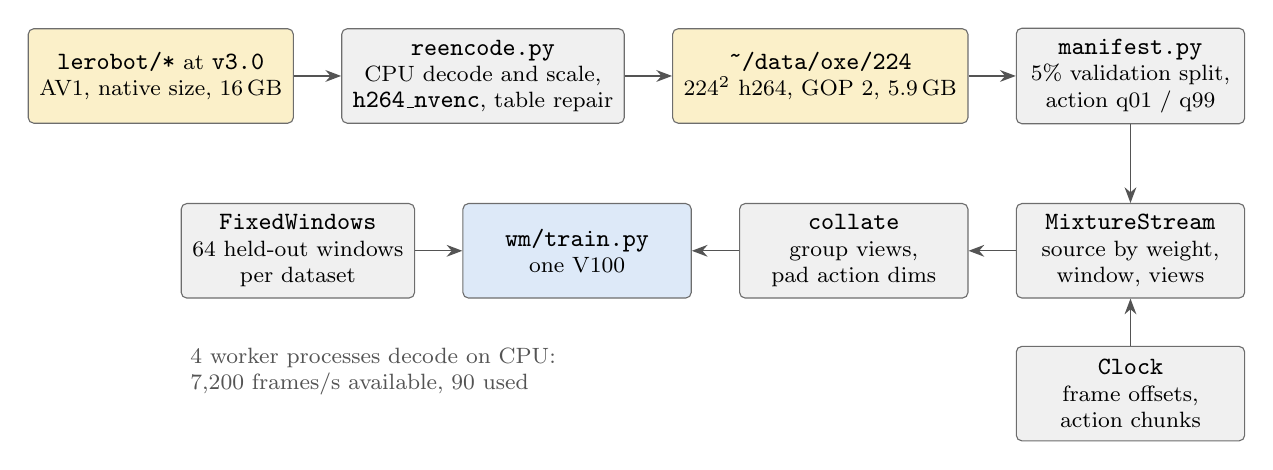
\begin{tikzpicture}[font=\footnotesize, node distance=5mm and 6mm,
  box/.style={draw=ink!60, rounded corners=2pt, fill=#1, align=center, inner sep=4pt, minimum height=12mm, minimum width=29mm},
  box/.default=white, arr/.style={-{Stealth[length=2mm]}, ink!70, line width=0.5pt}]
\node[box=store] (raw) {\code{lerobot/*} at \code{v3.0}\\AV1, native size, 16\,GB};
\node[box=proc, right=of raw] (re) {\code{reencode.py}\\CPU decode and scale,\\\code{h264\_nvenc}, table repair};
\node[box=store, right=of re] (out) {\code{\~{}/data/oxe/224}\\$224^2$ h264, GOP 2, 5.9\,GB};
\node[box=proc, right=of out] (man) {\code{manifest.py}\\5\% validation split,\\action q01 / q99};
\node[box=proc, below=10mm of man] (stream) {\code{MixtureStream}\\source by weight,\\window, views};
\node[box=proc, left=of stream] (col) {\code{collate}\\group views,\\pad action dims};
\node[box=model, left=of col] (train) {\code{wm/train.py}\\one V100};
\node[box=proc, left=of train] (val) {\code{FixedWindows}\\64 held-out windows\\per dataset};
\node[box=proc, below=6mm of stream] (clock) {\code{Clock}\\frame offsets,\\action chunks};
\draw[arr] (raw) -- (re); \draw[arr] (re) -- (out); \draw[arr] (out) -- (man);
\draw[arr] (man) -- (stream); \draw[arr] (clock) -- (stream); \draw[arr] (stream) -- (col);
\draw[arr] (col) -- (train); \draw[arr] (val) -- (train);
\node[ink!70, anchor=north west, align=left] at ($(val.south west)+(0,-5mm)$)
  {4 worker processes decode on CPU:\\7{,}200 frames/s available, 90 used};
\end{tikzpicture}
\caption{Data path. Yellow boxes are files on disk, grey boxes are code in
\code{thesis.mixture}, blue is the trainer. Re-encoding runs once; everything from the
manifest onward runs per training job. The validation windows come from the same
manifest's held-out episodes.}
\label{fig:pipeline}
\end{figure}

Eight real-robot datasets from the \code{lerobot/open-x-embodiment} collection, all at
revision \code{v3.0} (a tag, not a branch). Simulated sets (\code{usc\_cloth\_sim} and others)
were left out. \code{ucsd\_pick\_and\_place} has a dark, stylised look that could be
mistaken for a render, but it is the real xArm set; drop it from
\code{mixture.members} if you disagree after looking at the validation panels.

\begin{center}\small
\begin{tabular}{@{}lrrrlrrr@{}}
\toprule
Embodiment & fps & $K_e$ & $D_e$ & Cameras & Hours & Episodes & Weight \\
\midrule
taco\_play & 15 & 6 & 7 & static, gripper & 4.40 & 3{,}603 & 0.127 \\
jaco\_play & 10 & 4 & 4 & front, wrist & 2.17 & 1{,}085 & 0.089 \\
berkeley\_fanuc & 10 & 4 & 7 & front, wrist & 1.74 & 415 & 0.080 \\
utaustin\_mutex & 20 & 8 & 7 & front, wrist & 5.03 & 1{,}500 & 0.136 \\
ucsd\_pick\_place & 5 & 2 & 4 & front & 3.76 & 1{,}355 & 0.118 \\
stanford\_hydra & 10 & 4 & 7 & front, wrist & 9.95 & 570 & 0.192 \\
stanford\_robocook & 5 & 2 & 7 & four exterior & 6.28 & 2{,}460 & 0.152 \\
toto & 30 & 12 & 6 & front & 3.02 & 1{,}003 & 0.105 \\
\midrule
Total & & & & & 36.4 & 11{,}991 & \\
\bottomrule
\end{tabular}
\end{center}

The clock runs at $f_{wm}=2.5$\,Hz with 8 frames per window (2.8\,s, 7 transitions). 2.5\,Hz
divides every frame rate here, so no chunk is resampled in this run. Weights are
$\mathit{hours}^{0.5}$, normalised. 5\% of each dataset's episodes are held out.
Action semantics were set from the statistics, not from each dataset's documentation: all
are zero-mean deltas with a gripper channel, except \code{toto}, whose actions are absolute
targets (lag-1 autocorrelation 0.99) with a constant last dimension, which is dropped. With
per-embodiment projections and no resampling, a wrong \code{kind} label changes nothing in
this run.

\begin{figure}[H]
\centering
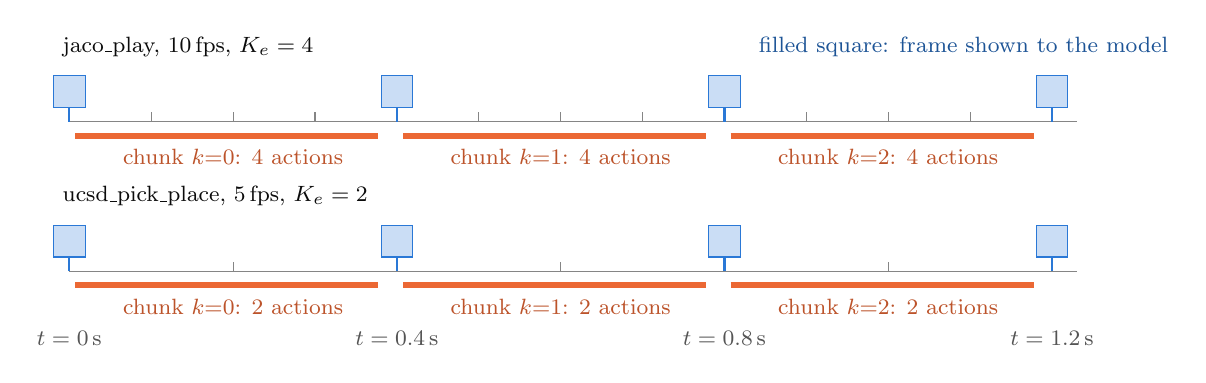
\begin{tikzpicture}[font=\footnotesize, x=5.2mm, y=1cm]
\foreach \row/\fps/\K/\n/\lab in {0/10/4/12/{jaco\_play, 10\,fps, $K_e=4$}, -1.9/5/2/6/{ucsd\_pick\_place, 5\,fps, $K_e=2$}} {
  \node[anchor=west, ink] at (-0.4, \row+0.95) {\lab};
  \draw[ink!50] (0,\row) -- (24.6,\row);
  \foreach \i in {0,...,\n} {
    \pgfmathsetmacro{\x}{\i*24/\n}
    \pgfmathtruncatemacro{\shown}{mod(\i,\K)==0}
    \ifnum\shown=1
      \node[draw=accent, fill=accent!25, minimum width=4mm, minimum height=4mm, inner sep=0] (f\i) at (\x,\row+0.38) {};
      \draw[accent, line width=0.8pt] (\x,\row) -- (\x,\row+0.17);
    \else
      \draw[ink!50] (\x,\row) -- (\x,\row+0.12);
    \fi
  }
  \foreach \k in {0,1,2} {
    \pgfmathsetmacro{\a}{\k*8+0.15}
    \pgfmathsetmacro{\b}{\k*8+8-0.15-24/\n}
    \pgfmathsetmacro{\m}{\k*8+4-12/\n}
    \draw[warm, line width=2.2pt] (\a,\row-0.18) -- (\b+24/\n-0.3,\row-0.18);
    \node[warm!80!black] at (\k*8+4,\row-0.45) {chunk $k{=}\k$: $\K$ actions};
  }
}
\foreach \k/\t in {0/0, 1/0.4, 2/0.8, 3/1.2} {
  \node[ink!70] at (\k*8, -2.75) {$t=\t$\,s};
}
\node[accent!70!black, anchor=west] at (16.6, 0.95) {filled square: frame shown to the model};
\end{tikzpicture}
\caption{The clock at $f_{wm}=2.5$\,Hz on two datasets with different frame rates. Both show
the model one frame every 0.4\,s. The action token for step $k$ is built from the native
actions between the frame shown at step $k$ and the frame shown at step $k{+}1$, so its
length $K_e$ differs by embodiment.}
\label{fig:clock}
\end{figure}

\subsection{A defect in the upstream v3.0 conversions}
On every camera stored in more than one video file, the episode table disagrees with the
files. When a video rolled over to a new file, the episode that crossed the size limit was
written at the start of the new file but recorded in the old file, with a start timestamp
past that file's end. Read as-is, 25 episode videos across five of the eight datasets point
at frames that do not exist (torchcodec raised \code{Invalid frame index=99701 ... must be
less than 99649}). The stock \code{LeRobotDataset} would hit the same episodes.

\code{reencode.py} now repairs this: an episode that starts at or past the end of its file is
moved to the next file with the overshoot as its offset, and the result must tile every file
exactly or the script raises. After the repair all 41 files tile exactly, and frame
differences confirm it: across each repaired boundary the mean absolute pixel change is 4 to
20 times the change inside the episode (hydra 68 vs.\ 6.5, toto 36 vs.\ 2.4, taco\_play 24
vs.\ 2.3).

\section{Re-encoding}
\paragraph{What the earlier sessions had found} (eryk-pc Claude chat of 1 November, wrist
camera of a b601 dataset): CPU decode and scale feeding NVENC, one \code{ffmpeg} per video,
was the fastest layout; GPU decode and \code{scale\_cuda} were slower and \code{scale\_cuda}
lost about 1.2\,dB; GPU decoding of h264 through torchcodec was unusable (5 samples/s), and
at $256{\times}256$ CPU decode matched GPU decode and kept its speed next to a training
loop. \code{h264\_nvenc} had failed to open and was set aside.

\paragraph{New here.}
\begin{itemize}
\item \textbf{\code{h264\_nvenc} fails only at GOP 1.} With \code{-g 1} the encoder refuses to
  open on this ffmpeg 6.1 and driver. From \code{-g 2} it works, so the requested
  $224{\times}224$ GOP-2 h264 runs on NVENC, 3.5 times faster than \code{libx264 -preset fast}
  (13.2\,s against 46.2\,s for 67{,}750 frames).
\item \textbf{AV1 decode is the bottleneck, not NVENC.} On one $320{\times}240$ file, decode
  alone runs at 4{,}290 frames/s and the full pipeline at 3{,}480. Changing the NVENC preset
  (p1 against p4) or the scaler (fast bilinear against bicubic) moved throughput by under
  2\%.
\item \textbf{One pool over all files of all datasets} (adopted). The first version ran
  one dataset at a time, which left cores idle on datasets with one or two files. Pooling
  everything, largest file first, two decode threads per process, sustained 7{,}960 frames/s
  over 1.9 million frames.
\item \textbf{Splitting a file into parallel segments} (measured, not adopted): 6{,}180
  frames/s on a lone file against 3{,}480, with exact frame counts. It only helps when there
  are fewer files than cores, which the pool already covers.
\end{itemize}

\begin{center}\small
\begin{tabular}{@{}lrl@{}}
\toprule
Variant (one hydra file, 97{,}352 frames, $320{\times}240$ AV1) & frames/s & Note \\
\midrule
NVENC p4, bicubic (baseline) & 3{,}484 & \\
NVENC p1, bicubic & 3{,}516 & same size \\
NVENC p4, fast bilinear & 3{,}543 & 35.7\,dB against baseline output \\
decode only & 4{,}290 & upper bound for one process \\
3 parallel segments & 5{,}064 & \\
10 parallel segments, 1 decode thread each & 6{,}175 & 47.7\,dB against baseline output \\
\bottomrule
\end{tabular}
\end{center}

All eight datasets (3.0 million video frames, 41 files) re-encoded in about 8 minutes of V100
time. The output is 5.9\,GB against about 16\,GB downloaded. \code{toto} was slowest
(2{,}680 frames/s) because its source is $640{\times}480$.

\section{Data loading}
Decoding is on CPU with torchcodec, in approximate seek mode, with decoders cached per
worker and one batched call per view. Measured on the eight-dataset mixture, 16 samples per
batch, up to two views per sample, 8 frames per view:

\begin{figure}[H]
\centering
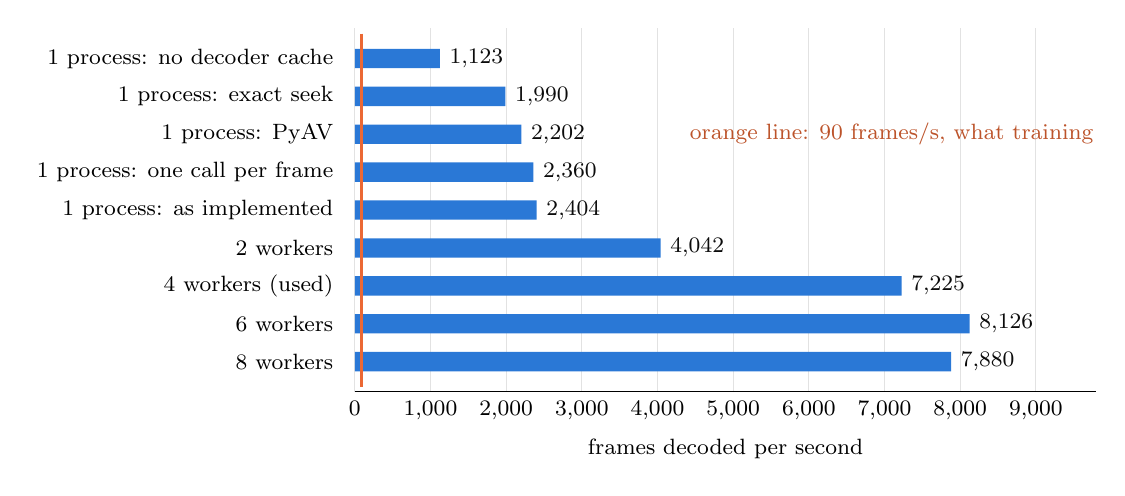
\begin{tikzpicture}
\begin{axis}[xbar, width=11cm, height=6.2cm, bar width=7pt, xmin=0, xmax=9800,
  axis x line*=bottom, axis y line*=left, y axis line style={draw=none}, tick style={draw=none},
  xmajorgrids, grid style={ink!12}, xlabel={frames decoded per second}, y dir=reverse,
  ytick=data, yticklabel style={font=\footnotesize, align=right}, xticklabel style={font=\footnotesize},
  label style={font=\footnotesize}, scaled x ticks=false,
  symbolic y coords={nocache,exact,pyav,perframe,one,w2,w4,w6,w8},
  yticklabels={1 process: no decoder cache, 1 process: exact seek, 1 process: PyAV, 1 process: one call per frame,
    1 process: as implemented, 2 workers, 4 workers (used), 6 workers, 8 workers},
  nodes near coords, nodes near coords style={font=\footnotesize, text=ink, anchor=west},
  point meta=explicit symbolic]
\addplot[fill=accent, draw=none] coordinates {(1123,nocache)[1{,}123] (1990,exact)[1{,}990] (2202,pyav)[2{,}202]
  (2360,perframe)[2{,}360] (2404,one)[2{,}404] (4042,w2)[4{,}042] (7225,w4)[7{,}225] (8126,w6)[8{,}126] (7880,w8)[7{,}880]};
\draw[warm, line width=1pt] ([yshift=9pt]axis cs:90,nocache) -- ([yshift=-9pt]axis cs:90,w8);
\node[warm!80!black, font=\footnotesize, anchor=west] at (axis cs:4300,pyav) {orange line: 90 frames/s, what training consumes};
\end{axis}
\end{tikzpicture}
\caption{Loader throughput on the eight-dataset mixture (16 samples per batch, up to two
views, 8 frames per view).}
\label{fig:loader}
\end{figure}


\begin{itemize}
\item The decoder cache is the one choice that matters (2.1 times). Exact seek mode costs 18\%
  in steady state and also scans each file on open.
\item Throughput stops scaling at 6 workers, the number of physical cores.
\item The model trains on about 90 frames/s, so loading is roughly 90 times faster than it
  needs to be. Training waits on data for under 0.1\% of a step with 4 workers. I did not
  optimise further; with a ViT-S encoder or four GPUs the loader would start to matter, and
  the first thing to try then is a GOP-1 or JPEG-per-frame store to remove the one extra
  decoded frame per request.
\end{itemize}

\section{Model and training setup}
\begin{figure}[H]
\centering
\begin{adjustbox}{max width=\linewidth}
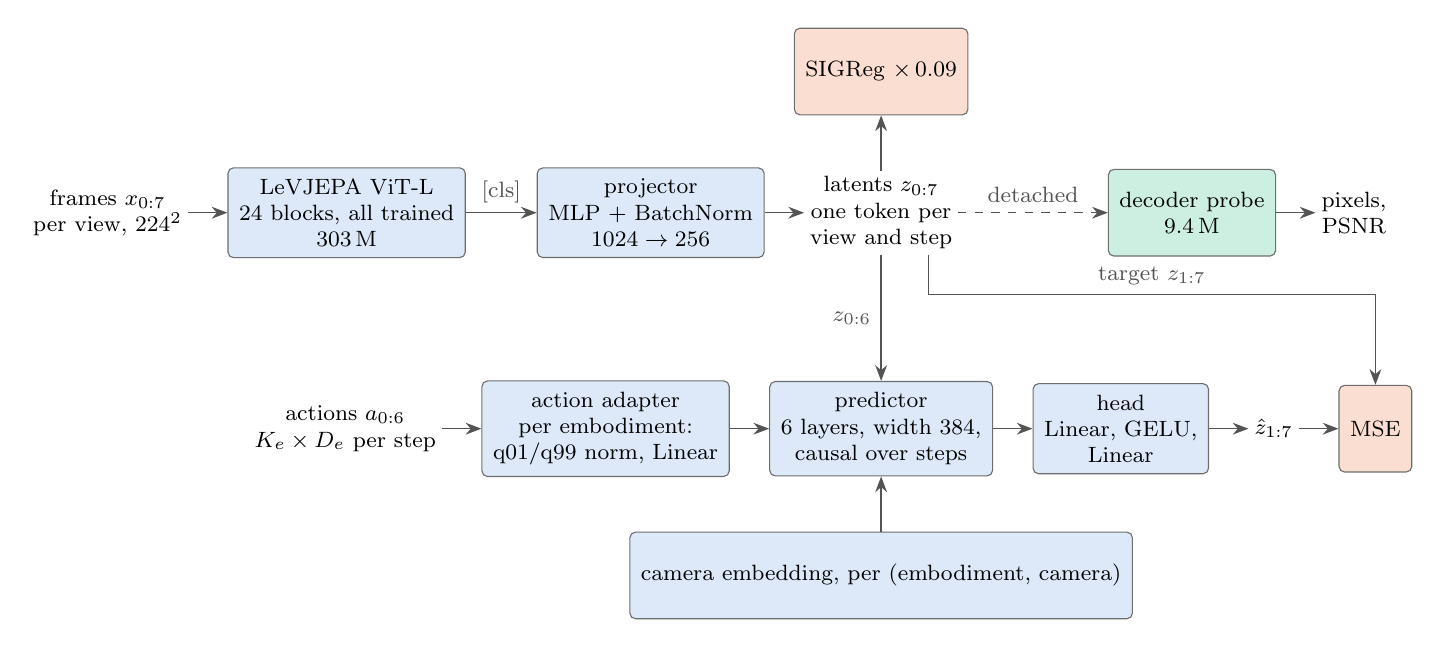
\begin{tikzpicture}[font=\footnotesize, node distance=5mm and 5mm,
  box/.style={draw=ink!60, rounded corners=2pt, fill=#1, align=center, inner sep=4pt, minimum height=11mm},
  box/.default=white, io/.style={align=center, inner sep=2pt},
  arr/.style={-{Stealth[length=2mm]}, ink!70, line width=0.5pt},
  det/.style={-{Stealth[length=2mm]}, ink!70, line width=0.5pt, dashed}]
\node[io] (x) {frames $x_{0:7}$\\per view, $224^2$};
\node[box=model, right=of x] (enc) {LeVJEPA ViT-L\\24 blocks, all trained\\303\,M};
\node[box=model, right=9mm of enc] (proj) {projector\\MLP + BatchNorm\\$1024\rightarrow256$};
\node[io, right=of proj] (z) {latents $z_{0:7}$\\one token per\\view and step};
\node[box=loss, above=7mm of z] (sig) {SIGReg $\times\,0.09$};
\node[box=probe, right=19mm of z] (dec) {decoder probe\\9.4\,M};
\node[io, right=of dec] (img) {pixels,\\PSNR};
\node[box=model, below=16mm of z] (pred) {predictor\\6 layers, width 384,\\causal over steps};
\node[box=model, left=of pred] (act) {action adapter\\per embodiment:\\q01/q99 norm, Linear};
\node[io, left=of act] (a) {actions $a_{0:6}$\\$K_e\times D_e$ per step};
\node[box=model, below=7mm of pred] (cam) {camera embedding, per (embodiment, camera)};
\node[box=model, right=of pred] (head) {head\\Linear, GELU,\\Linear};
\node[io, right=of head] (zh) {$\hat z_{1:7}$};
\node[box=loss, right=of zh] (mse) {MSE};
\draw[arr] (x) -- (enc); \draw[arr] (enc) -- node[above, ink!70]{[cls]} (proj); \draw[arr] (proj) -- (z);
\draw[arr] (z) -- node[left, ink!70]{$z_{0:6}$} (pred); \draw[arr] (pred) -- (head); \draw[arr] (head) -- (zh); \draw[arr] (zh) -- (mse);
\draw[arr] (a) -- (act); \draw[arr] (act) -- (pred); \draw[arr] (cam) -- (pred);
\draw[arr] (z) -- (sig);
\draw[arr] ($(z.south)+(6mm,0)$) -- ++(0,-5mm) -| node[pos=0.25, above, ink!70]{target $z_{1:7}$} (mse.north);
\draw[det] (z) -- node[above, ink!70]{detached} (dec); \draw[arr] (dec) -- (img);
\end{tikzpicture}
\end{adjustbox}
\caption{The model. Blue blocks are trained by the two losses in orange, with no
stop-gradient and no EMA target. The decoder probe (green) reads detached latents, so it
never shapes them. The head is the block that used to contain a BatchNorm
(Section~\ref{sec:bn}).}
\label{fig:arch}
\end{figure}

\begin{itemize}
\item \textbf{Encoder:} LeVJEPA VideoMix ViT-L (303\,M parameters), fully unfrozen, one
  frame per clip, [cls] output. A BatchNorm projector maps it to a 256-d latent: one token
  per camera per step.
\item \textbf{Actions:} per embodiment, the $K_e \times D_e$ chunk is normalised with that
  embodiment's 1st and 99th percentiles and projected by its own linear layer to one token.
\item \textbf{Predictor:} 6-layer, 384-wide causal transformer. Per step it reads each
  view's latent plus a learned per-(embodiment, camera) embedding, and the action token; the
  output at a view's token is that view's latent at the next step. 14.8\,M parameters with
  the projectors (Figure~\ref{fig:tokens}).
\item \textbf{Loss:} next-latent MSE plus $0.09\times$SIGReg on all latents of the batch, as
  in LeWorldModel. No stop-gradient, no EMA. The prediction head has no BatchNorm, unlike
  LeWorldModel's (Section~\ref{sec:bn}).
\item \textbf{Probe:} a cross-attention pixel decoder (9.4\,M) trained on detached latents
  only. It is never trained on predicted latents.
\item \textbf{Optimisation:} AdamW, encoder lr $2\times10^{-5}$, everything else
  $3\times10^{-4}$, 500 warm-up steps then cosine to 10\%, fp16, gradient clip 1.0, batch 16
  samples (about 28 views, 225 frames).
\end{itemize}

\begin{figure}[H]
\centering
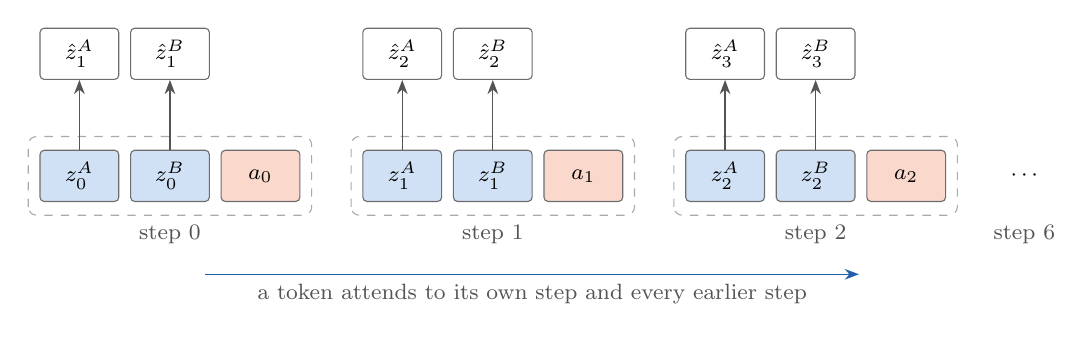
\begin{tikzpicture}[font=\footnotesize, x=1cm, y=1cm,
  tok/.style={draw=ink!60, rounded corners=1.5pt, minimum width=10mm, minimum height=6.5mm, inner sep=0, fill=#1},
  arr/.style={-{Stealth[length=1.8mm]}, ink!70, line width=0.5pt}]
\foreach \s in {0,1,2} {
  \pgfmathsetmacro{\o}{\s*4.1}
  \pgfmathtruncatemacro{\sn}{\s+1}
  \node[tok=accent!22] (v\s) at (\o,0) {$z^{A}_{\s}$};
  \node[tok=accent!22] (w\s) at (\o+1.15,0) {$z^{B}_{\s}$};
  \node[tok=warm!25] (a\s) at (\o+2.3,0) {$a_{\s}$};
  \draw[ink!35, dashed, rounded corners=3pt] (\o-0.65,-0.5) rectangle (\o+2.95,0.5);
  \node[ink!70] at (\o+1.15,-0.75) {step \s};
  \node[tok=white] (p\s) at (\o,1.55) {$\hat z^{A}_{\sn}$};
  \node[tok=white] (q\s) at (\o+1.15,1.55) {$\hat z^{B}_{\sn}$};
  \draw[arr] (v\s) -- (p\s); \draw[arr] (w\s) -- (q\s);
}
\node at (12.0,0) {$\cdots$}; \node[ink!70] at (12.0,-0.75) {step 6};
\draw[arr, accent!80!black] (1.6,-1.25) -- node[below, ink!70]{a token attends to its own step and every earlier step} (9.9,-1.25);
\end{tikzpicture}
\caption{Predictor sequence for a two-camera sample: 7 steps of (view, view, action), 21
tokens. The output at a view's token is that view at the next step. A sample with one camera leaves its second slot empty and masked out of attention.
The frozen and unfrozen runs both use this layout.}
\label{fig:tokens}
\end{figure}

\paragraph{Fitting an unfrozen ViT-L on a 16\,GB V100.}
\begin{center}\small
\begin{tabular}{@{}lrrrr@{}}
\toprule
Encoder training & Samples & Frames/step & s/step & Peak memory \\
\midrule
all 24 blocks, gradient checkpointing & 12 & 192 & 2.17 & 10.4\,GiB \\
all 24 blocks, gradient checkpointing & 16 & 256 & 2.84 & 11.7\,GiB \\
all 24 blocks, gradient checkpointing & 20 & 320 & 3.57 & 13.1\,GiB \\
last 12 blocks, gradient checkpointing & 32 & 512 & 3.59 & 12.2\,GiB \\
any setting without checkpointing & $\geq 8$ & & & out of memory \\
\bottomrule
\end{tabular}
\end{center}
(Worst case, two views for every sample.) Full unfreezing trains about 90 frames/s; the last
12 blocks alone, 143. The run below uses all 24 blocks at 16 samples. The encoder is the whole
cost: the predictor sees 21 tokens per sample.

\section{Results of the test run}
Four runs, all with seed 0 and the same data order. Each validation pass uses 64 fixed
held-out windows per dataset (512 in total): the model is given 3 true frames and all
actions, then rolls out 5 steps on its own predictions.

\begin{center}\small
\begin{tabular}{@{}llllr@{}}
\toprule
Run & Encoder & Prediction head & GPU & Steps \\
\midrule
\code{oxe\_small\_v1} & trained & MLP + BatchNorm (LeWM) & V100 & 5{,}400 (cancelled) \\
\code{oxe\_small\_frozen} & frozen & MLP + BatchNorm (LeWM) & RTX 2060 & 6{,}000 \\
\code{oxe\_small\_v2} & trained & MLP, no BatchNorm & V100 & 4{,}500 \\
\code{oxe\_small\_frozen\_v2} & frozen & MLP, no BatchNorm & RTX 2060 & 4{,}500 \\
\bottomrule
\end{tabular}
\end{center}

\subsection{Stability}
The unfrozen run with the plain head trains without incident (Figure~\ref{fig:train}). The
latent standard deviation reaches 0.97 by step 1{,}000 and stays there, the SIGReg
statistic falls from 60 to about 3.6, and the training prediction error falls below the
copy baseline from about step 900 on. No step was skipped for a non-finite loss after the first
25. A step takes 2.6\,s, so 4{,}500 steps is about 3.3 hours.

\begin{figure}[H]
\centering
\includegraphics[width=\linewidth]{wm_report_figures/train_unfrozen.pdf}
\caption{Training curves of the unfrozen run with the plain head (\code{oxe\_small\_v2}).}
\label{fig:train}
\end{figure}

\subsection{Prediction quality}
\begin{center}\small
\begin{tabular}{@{}lrr@{}}
\toprule
Held-out, all datasets, step 4{,}500 & Encoder trained & Encoder frozen \\
\midrule
One-step latent MSE, predictor & 0.049 & 0.076 \\
One-step latent MSE, copy last latent & 0.139 & 0.109 \\
Rollout step 5 latent MSE, predictor & 0.202 & 0.184 \\
Rollout step 5 latent MSE, copy & 1.000 & 0.463 \\
\midrule
PSNR, decode of the true latent (dB) & 17.12 & 17.44 \\
PSNR, rollout step 1 / copy (dB) & 17.03 / 16.89 & 17.34 / 17.25 \\
PSNR, rollout step 5 / copy (dB) & 16.71 / 16.10 & 17.11 / 16.56 \\
\bottomrule
\end{tabular}
\end{center}

\begin{itemize}
\item \textbf{Both models beat copying, at one step and over the rollout.} Five steps out,
  the rollout decodes 0.5 to 0.6\,dB above the copied frame in both runs
  (Figure~\ref{fig:val}).
\item \textbf{Latent errors cannot be compared between the two columns.} Each run has its own
  latent space. In the unfrozen run the copy error itself rises from 0.076 to 0.139 as the
  encoder trains, which means consecutive latents move further apart; the predictor's
  advantage over copying (ratio 0.35 against 0.70 frozen) partly reflects that.
\item \textbf{In pixels the frozen encoder is slightly ahead} (17.44 against
  17.12\,dB for decoding the true latent). Each run has its own probe, both probes were
  still improving, and this is one seed, so I would not read a ranking into 0.3\,dB.
\item \textbf{The predictor is close to the probe's ceiling.} Rollout step 5 is 0.3 to 0.4\,dB
  below the decode of the true latent. The probe, and what one token holds, limit the
  number more than the dynamics do.
\end{itemize}

\begin{figure}[H]
\centering
\includegraphics[width=\linewidth]{wm_report_figures/val_unfrozen.pdf}
\caption{Held-out curves of the unfrozen run with the plain head.}
\label{fig:val}
\end{figure}

\begin{figure}[H]
\centering
\includegraphics[width=\linewidth]{wm_report_figures/compare_v2.pdf}
\caption{Trained against frozen encoder, both with the plain head. Left: below 1 beats
copying. Middle: above 0 beats copying.}
\label{fig:cmp}
\end{figure}

\paragraph{Per dataset.} The unfrozen model beats copying on all eight datasets in latent
error (Figure~\ref{fig:peremb}). The pixel gain is largest where the camera or arm moves
most within 2\,s (\code{ucsd\_pick\_place} +1.3\,dB, \code{utaustin\_mutex} +1.2\,dB,
\code{taco\_play} +0.9\,dB) and is under 0.1\,dB on \code{toto} and
\code{stanford\_robocook}, where the frame barely changes.

\begin{figure}[H]
\centering
\includegraphics[width=\linewidth]{wm_report_figures/per_emb_unfrozen.pdf}
\caption{Per-dataset results of the unfrozen run at step 4{,}500.}
\label{fig:peremb}
\end{figure}

\subsection{What the decodes look like}
Figure~\ref{fig:panels} shows one held-out window per dataset. The probe produces close to
one colour per 16-pixel patch, so a decode is a $14\times14$ colour layout of the scene. The
robot arm is visible as a blob where it is large and bright (\code{ucsd\_pick\_place},
\code{stanford\_hydra}) and not otherwise, and small objects are absent. Rollout rows are
nearly indistinguishable from the decode of the true latent. About 17\,dB is therefore a
statement about background layout. I have not checked whether the blockiness comes from the
probe (4 layers, trained for the same few thousand steps) or from what the single token
keeps; a longer probe fit on a frozen checkpoint would separate the two.

\newcommand{\panel}[2]{%
  \begin{minipage}[t]{0.485\linewidth}\centering
  \includegraphics[width=\linewidth]{wm_report_figures/panel_unfrozen_#1.jpg}\\[-1pt]
  {\footnotesize #2}\end{minipage}}
\begin{figure}[H]
\centering
\panel{taco_play}{taco\_play}\hfill\panel{jaco_play}{jaco\_play}\\[5pt]
\panel{berkeley_fanuc}{berkeley\_fanuc}\hfill\panel{utaustin_mutex}{utaustin\_mutex}\\[5pt]
\panel{ucsd_pick_place}{ucsd\_pick\_place}\hfill\panel{stanford_hydra}{stanford\_hydra}\\[5pt]
\panel{stanford_robocook}{stanford\_robocook}\hfill\panel{toto}{toto}
\caption{Held-out rollouts of the unfrozen model at step 4{,}500, one window per dataset.
In each block the columns are the 5 rollout steps (0.4\,s apart) and the rows are, top to
bottom: the true frame, the probe's decode of the true latent, and the probe's decode of
the rolled-out latent.}
\label{fig:panels}
\end{figure}

\subsection{The BatchNorm in the prediction head}
\label{sec:bn}
LeWorldModel puts a BatchNorm MLP after the encoder (the projector) and another after the
predictor (the prediction head). The first unfrozen run used both. Its training error
looked fine (0.05 against 0.16 for copying), but its validation error, measured in eval
mode, rose from 0.15 to 0.92 and rollouts reached a latent error of 13 against 1 for
copying (Figure~\ref{fig:bncmp}). The frozen run with the same head had no such problem.

\begin{figure}[H]
\centering
\includegraphics[width=\linewidth]{wm_report_figures/compare_bn.pdf}
\caption{The two runs with LeWM's BatchNorm head, and the unfrozen run with the plain head.
The left panel is on a linear scale, so the blue curve leaving the top is the failure.}
\label{fig:bncmp}
\end{figure}

To locate it I evaluated one checkpoint of that run four ways
(\code{bench/bn\_diag.py}, Figure~\ref{fig:bn}). Switching the projector between batch and
running statistics changes little. Switching the head does everything: 0.049 with batch
statistics, 0.255 with running statistics. On the frozen checkpoint the two modes agree
(0.078 and 0.089).

\begin{figure}[H]
\centering
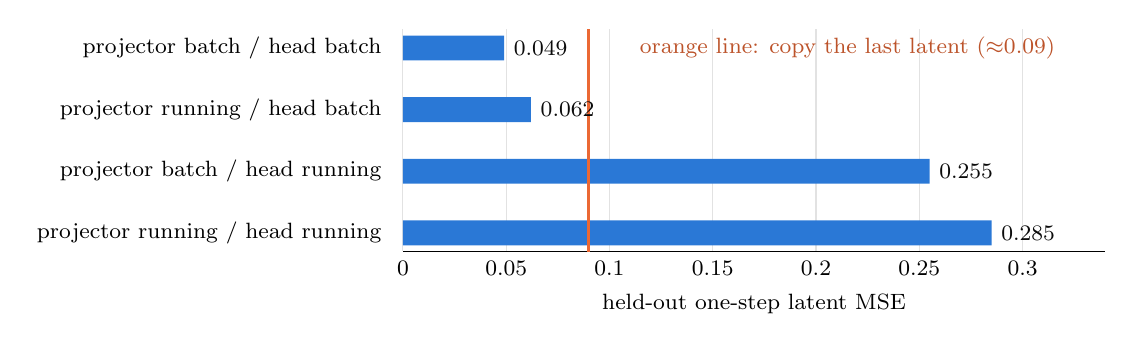
\begin{tikzpicture}
\begin{axis}[xbar, width=10.5cm, height=4.4cm, bar width=9pt, xmin=0, xmax=0.34,
  axis x line*=bottom, axis y line*=left, y axis line style={draw=none}, tick style={draw=none},
  xmajorgrids, grid style={ink!12}, xlabel={held-out one-step latent MSE}, y dir=reverse,
  ytick=data, yticklabel style={font=\footnotesize}, xticklabel style={font=\footnotesize, /pgf/number format/fixed},
  label style={font=\footnotesize},
  symbolic y coords={bb,rb,br,rr},
  yticklabels={projector batch / head batch, projector running / head batch, projector batch / head running, projector running / head running},
  nodes near coords, nodes near coords style={font=\footnotesize, text=ink, /pgf/number format/fixed, /pgf/number format/precision=3, anchor=west}]
\addplot[fill=accent, draw=none] coordinates {(0.049,bb) (0.062,rb) (0.255,br) (0.285,rr)};
\draw[warm, line width=1pt] ([yshift=11pt]axis cs:0.09,bb) -- ([yshift=-11pt]axis cs:0.09,rr);
\node[warm!80!black, font=\footnotesize, anchor=west] at (axis cs:0.11,bb) {orange line: copy the last latent ($\approx$0.09)};
\end{axis}
\end{tikzpicture}
\caption{The first unfrozen run's checkpoint, evaluated on the same held-out windows with
each BatchNorm using either the statistics of the batch or its running averages. Only the
prediction head's setting matters.}
\label{fig:bn}
\end{figure}


\paragraph{What I changed.} \code{WorldModel.pred\_proj} is now Linear, GELU, Linear. The
predictor's output is already layer-normalised. The projector keeps its BatchNorm, so the
latent that SIGReg acts on is produced exactly as in LeWM. With this head, held-out error
follows training error and rollouts are stable (the green curve in
Figure~\ref{fig:bncmp}).

\paragraph{What I do not know.} Why the head came to depend on batch statistics when the
encoder trains. I tested no mechanism. A model that needs batch statistics at inference
cannot be used for planning, where the batch is a set of candidate action sequences from
one state, so some fix was needed, but I did not try the alternatives that stay closer to
LeWM: a LayerNorm in the head, a lower BatchNorm momentum, or recomputing the running
statistics after training. The original runs are kept in \code{runs/oxe\_small\_v1} and
\code{runs/oxe\_small\_frozen}.


\section{Limits of this run and what I would do next}
\paragraph{Limits.}
\begin{itemize}
\item One seed, 4{,}500 steps, batch 16. That is 72{,}000 windows. Every curve was still improving when the runs ended.
\item PSNR through a small probe that renders patch-level colour says little about whether
  the latent tracks the robot. A probe that reads out end-effector state from the latent
  would test that directly, and state is already in the batch.
\item The frozen control ran on the RTX 2060 and the unfrozen run on the V100. Same seed
  and data order, but the comparison is two single runs.
\item No planning or policy evaluation was attempted, as agreed.
\item Action semantics were inferred from statistics. That is harmless with per-embodiment
  projections and would matter as soon as actions are shared or converted.
\end{itemize}

\paragraph{Next, in the order I would do them.}
\begin{enumerate}
\item Decide the head: run the LayerNorm variant against the plain head, and make the choice
  a config option. This is the one place the model departs from LeWM.
\item Fit a larger probe for longer on the two final checkpoints, to learn whether 17\,dB is
  the probe or the token.
\item Add a state read-out probe.
\item A longer run (20{,}000 steps or more) at the last-12-blocks setting, which trains 1.6
  times more frames per second.
\item Commit the branch. Nothing is committed yet.
\end{enumerate}

\paragraph{Commands.}
\begin{verbatim}
cd ~/School/thesis/scratch/multiemb/repo
sbatch scripts/local/oxe_reencode.sbatch
sbatch scripts/local/wm_train.sbatch configs/wm/oxe_small.yaml
python scripts/plot_wm_run.py <run_dir> <out_dir>
\end{verbatim}


\end{document}
